\documentclass{standalone}
\usepackage[dvipsnames,svgnames,x11names]{xcolor}
\usepackage{tikz}
\usepackage{pgfplots}
\pgfplotsset{compat = 1.12}
\usepackage{../thesismath}
\begin{document}
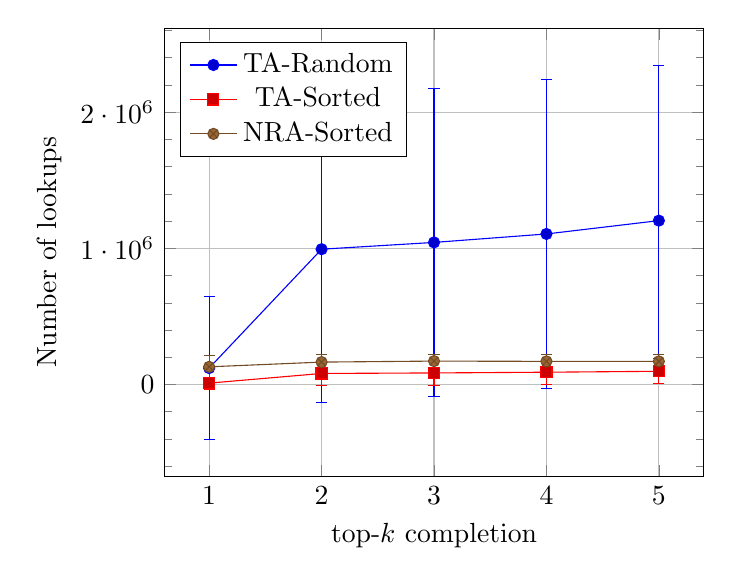
\begin{tikzpicture}[baseline]

\begin{axis}[
  xlabel = {top-$k$ completion},
  xtick = {1, ..., 5},
  ylabel = {Number of lookups},
  scaled ticks = false,
  %y tick label style={/pgf/number format/fixed},
  %ymin = -150000,
  %ymax = 1300000,
  minor y tick num = 4,
  grid = major,
  legend entries = {{TA-Random}, {TA-Sorted}, {NRA-Sorted}},
  legend pos = north west,
]

% over 100 test sequences on my own machine

% TA-GLM-Random
\addplot+[
  error bars/.cd,
  y dir = both,
  y explicit,
] table [y error = num_error] {
  n num     num_error
  1  120563  522428
  2  993536 1123401
  3 1043303 1133535
  4 1105481 1132395
  5 1203434 1138707
};

% TA-GLM-Sorted
\addplot+[
  error bars/.cd,
  y dir = both,
  y explicit,
] table [y error = num_error] {
  n num      num_error
  1    9861   43274
  2   80870   90819
  3   84661   91325
  4   89961   91416
  5   96874   90906
};

% NRA-GLM-Sorted
\addplot+[
  error bars/.cd,
  y dir = both,
  y explicit,
] table [y error = num_error] {
  n num      num_error
  1  129616   85141
  2  164360   58803
  3  171719   48627
  4  169696   51421
  5  169641   51237
};

\end{axis}

\end{tikzpicture}
\end{document}
